	Avant le début de ce projet, la banque Neuflize OBC (nous abrégerons maintenant NOBC) possédait déjà un site web mis à disposition de ses clients. Celui-ci à été réalisé par NOBC qui a fait le choix de faire appel à EFS pour construire son back end. Comme nous l'avons déjà dit, EFS est une prestataire et éditeur de la solution \textit{Webank} proposant de nombreux services grandement sécurisés permettant de faire de l'authentification, de la signature de transactions numériques etc... NOBC a donc développé un back end pouvant communiquer avec ces services via le transfert de \textit{fichiers} contenant les données à persister. EFS dispose de ses propres bases afin de persister lesdits fichiers. La communication est donc bidirectionnelle puisque le back end interne de NOBC (le \textit{core banking}) doit impérativement maintenir ses bases de données internes à jour. Ainsi, une synchronisation des fichiers a lieue une fois par jour afin d'actualiser les bases et d'assurer la cohérence. Il est possible d'observer les actions entres les différents acteurs sur le schéma figure \ref{archiFonc}. \\
	
	Cependant, dans le cadre d'une application mobile, il n'était pas possible d'interroger directement EFS de la même manière que pour le web. En effet, pour des raisons de performances, il est grandement conseillé, sur mobile, d'essayer de faire correspondre un écran avec un seul service. Cela permet de d'améliorer la fluidité lors de la navigation sur l'application. C'est pourquoi une couche d'\textit{API microservices} a été développée afin de réaliser la composition des services EFS afin de répondre à ce besoin. Pour cela, il a été demandé à EFS de mettre en place une \textit{surcouche} afin d'exposer ses services et transmettre les réponses via le format de données JSON et non plus directement via du SQL. La communication entre EFS et l'API microservices étant établie, il fallait maintenant sécuriser l'accès à la couche microservices. Afin de ne pas réinventer la roue et d'obtenir un résultat optimal en fonction du coût du projet, il a été décidé de mettre en place une couche \textit{API Gateway} basé sur l'API d'Axway, une filiale de Sopra Steria (cette couche sera décrite plus en détails dans la partie \ref{axway}). \\
	
	Enfin, une fois la gateway mise en place, cette dernière est devenue le point d'entrée du projet. Elle reçoit les requêtes depuis la \textit{Rest Layer} mis en place par l'équipe chargée du développement du front end de l'application, à savoir PBI, qui est notre client et qui consomme nos microservices. \\

	L'API microservices utilise la stack Netflix OSS qui permet d'intégrer les patterns classiques aux application distribuées. Les composants Netflix sont intégrés via Spring Cloud. Les services proposés par cette couche sont les suivants :\\

\begin{itemize}
			\item account-service : gérant les informations liées aux comptes des utilisateurs
			\item profile-service : gérant les informations liées aux profils des utilisateurs
			\item transaction-service : gérant les informations liées aux transactions bancaires \\
\end{itemize}

	Ces services permettent de fournir de nombreuses fonctionnalités de consultation et de transaction. Voici une liste des principales fonctionnalités associées au service correspondant :
	\begin{itemize}
		\item TODO
		\item Consultation des comptes bancaires (montant, etc...)
		\item Rib
		\item Opérations bancaires sur le compte
		\item Transactions réalisées/reçues
		\item Initier une transaction
		\item Signer numériquement une transaction
		\item Authentification par clavier virtuel
		\item Rechercher les comptes créditeurs
		\item Rechercher les comptes débiteurs
	\end{itemize}

\begin{figure}[H]
\raggedleft
	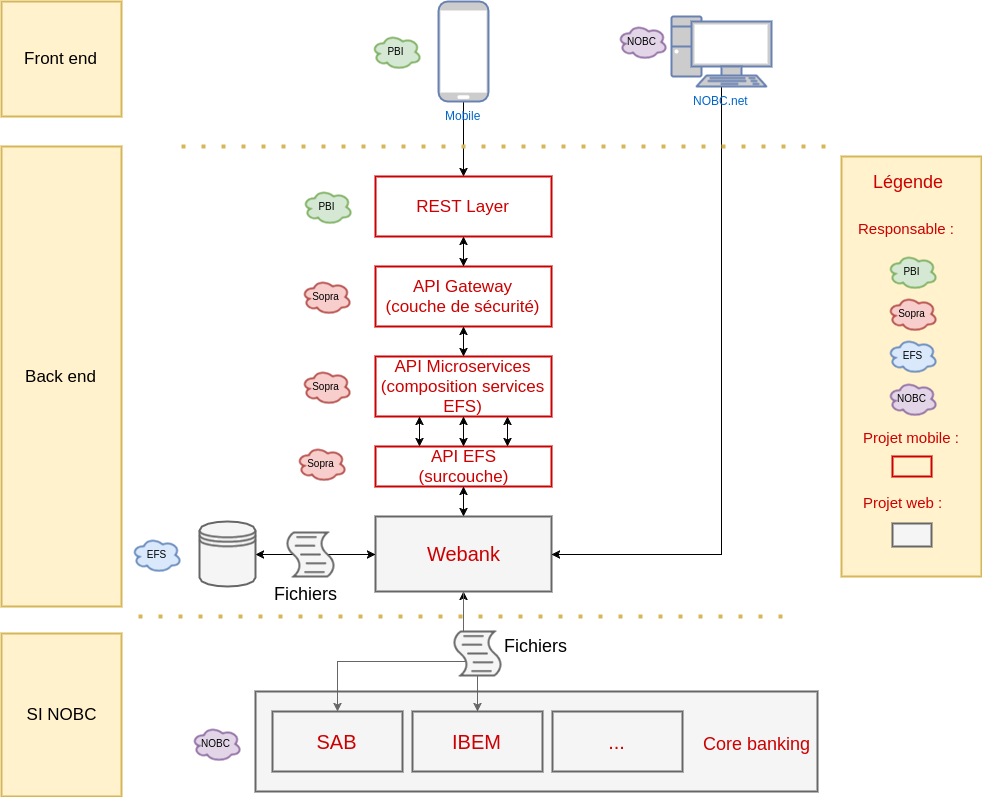
\includegraphics[scale=0.45]{images/travailNeuflizeOBC/architecture/archiFonc.png}
	\centering
	\caption{Présentation du projet et des acteurs}
	\label{archiFonc}
\end{figure}

